\subsection{Oryantalist Resim ve Ağırlık Koleksiyonu}
\indent\indent Müzenin ikinci katında, 17. yüzyıldan 20. yüzyıl başlarına uzanan bir dönemi kapsayan eserler sergilenmektedir. Bu koleksiyonda, Avrupalı ressamların Osmanlı dünyasını ve Türkiye coğrafyasını betimleyen yapıtlarının yanı sıra, Osmanlı sanatçılarının bu dönemdeki karşılıklı etkileşimleri yansıtan eserlerine de yer verilmektedir. İmparatorluğun son iki yüzyılına dair geniş bir görsel panorama sunan bu bölümde, Osman Hamdi Bey’in eserleri ile ünlü \textit{Kaplumbağa Terbiyecisi} adlı tablosu da bulunmaktadır.\newline
\indent \textit{Elçi Alayı}, dört adet tablodan oluşan ve Flaman asıllı Fransız ressamı Jean Baptiste Vanmour tarafından resmedilmiş eserdir. Vanmour, 1699 yılında İstanbul’a Fransız elçi Ferriol ile birlikte gelmiş ve Osmanlı toplumuna dair detaylı figüratif betimlemeler yapmıştır. İlk tabloda elçi alayının Galata sırtlarından Haliç'e inişi resmedilmiştir. Elçi Alayı'nın geçtiği yer, günümüzde Pera Müzesi'nin önündeki Meşrutiyet Caddesi'dir. İkinci tabloda ise alayın Topkapı Sarayı'na teşrifi anlatılmıştır. Tablodan kabulün ulufe divanı ile birşeştirlmiş bir elçi divanında, yani büyük divanda yapıldığını anlamaktayız. Alayın Bab-ı Hümayun'dan giriş yaptığı sırada, elçi heyetini etkilemek için yapılan Çanak Yağması ikinici tablodaki ilginç detaylardan biridir. Üçüncü tabloda ise, heyet şerefine Kubbealtı'nda verilen yemek bulunmaktır. Burada, Kasr-ı Adl adlı kafeste III.Ahmed'in gölgesini görmekteyiz. Dördünce tabloda ise, heyetin padişah III.Ahmed tarafından kabulu anlatılmıştır. \newline
\indent Buradaki en eski eser ise, Kutsal Roma İmparatoru II. Ferdinand tarafından Osmanlı İmparatoru 4. Murad'a elçi olarak gönderilen Hans Ludwig von Kuefstein’in elçilik heyetinde olan Avusturyalı ressamlar Franz Hermann, Hans Gemminger ve Hermann'ın yardımcısı olduğu anlaşılan Valentin Mueller tarafından yapılan 1654 tarihli \textit{Türk Hareminden Bir Sahne} isimli bir tablodur. Ters perspektif şeklinde resmedilmiş olan eserde, ön kısımdaki kompozisyon haremde misafir karşılama ve dans teması işlenmiştir. Arkadakı kompozisyonda da haremin bir odası tasvir edilmiştir. Resmi yapan kişilerin haremi görme şansı olmadığından, tablo büyük bir ihtimalle harem hakkında duyduklarının ve öğrendiklerinin yansımasıdır. Resimdeki halı motiflerinin daha İran tarzı olması belki de bundandır.\newline
\indent Koleksiyondaki en değerli eser aynı zamanda bir Türk tarafından yapılmış en pahalı tablo olup, 2003 yılında bir müzayedede 3.5milyon dolara alınmış olan Osman Hamdi Bey'in \textit{Kaplumbağa Terbiyecisi} isimli tablosudur. Osman Hamdi Bey, Paris'teki eğitimi sırasında resim dersleri almış ve batı resmini oryantal öğelerle harmanlayarak Türkiye resim sanatında yeni bir dönem başlatmıştır. Müzenin bu kısmında Kaplumbağa Terbiyecisi ile birlikte dört tane daha eseri sergilenmektedir.\newline
\indent Tablonun resimlediği sahnede yerdeki yeşillikleri yemekte olan kaplumbağaları düşünceli bir tavırla izleyen Doğulu giysiler içinde bir Osman Hamdi Bey'in otoportresini görürüz.  Elinde bir ney tutmakta, sırtında nakkare veya kudüm cinsinden bir vurmalı çalgı durmaktadır. Önünde durduğu pencerenin üstünde yer alan sivri kemerli alınlıkta \textit{Şifa’al-kulûp lika’al Mahbub} yani \textit{Kalplerin şifası, Sevgiliyle (Hz. Muhammed) buluşmaktır} yazılıdır. Mekân olarak, sanatçının resimlerinde sıkça karşımıza çıkan Bursa Yeşil Cami’nin hünkar mahfili kullanılmıştır. Adamın elinde, sırtında yer alan çalgılar derviş olabileceğini akla getirse de, başlığı Elbise-i Osmaniye’de yemeniler dolanmış keçe kalpak olarak tanımlanan \textit{Mardinli Kürd} tipinin başlığına benzer. Eser, Türkiye'nin tembel ve umursamaz bürokrasisine bir eleştiri niteliğindedir. Kaplumbağalar, yavaş ve içine kapanık bir hayvan olduğu için bürokrasinin tembelliğini ve tepkisizliğini simgelemektedir. Eserin merkezinde adam ise kaplumbağaları müzik(sanat) ile eğitmeyi denemektedir. Bezgin bir halde resmedilmiş adamın yüzünden muvaffak olamadığını anlıyoruz. Kaplumbağa Terbiyecisi, Osman Hamdi Bey’in koleksiyondaki beş eserinden biridir.\newline
\indent Müzenin ilk katı, prehistorik çağlardan günümüze Anadolu coğrafyasında gündelik hayatın tanıklığını yapmış objelere ev sahipliği yapıyor. Koleksiyon prehistorik dönem, Klasik Dönem, Beylikler ve Osmanlı Dönemi ile Erken Cumhuriyet dönemi başta olmak üzere Anadolu’nun ev sahipliği yaptığı birçok uygarlığa ait materyal bulunmaktadır. Arazi ölçümünden her türlü alışverişe, mimarlıktan kuyumculuğa, denizcilikten eczacılığa, astronomiden zaman ölçüm aletlerine kadar farklı alanlardan birçok ağırlık, uzunluk, hacim ölçüsünü bünyesinde barındıran bu koleksiyon Anadolu’nun zengin ve çok çeşitli kültürüne tarihsel bir perspektif sunmaktadır.
\begin{figure}[H]
    \centering
    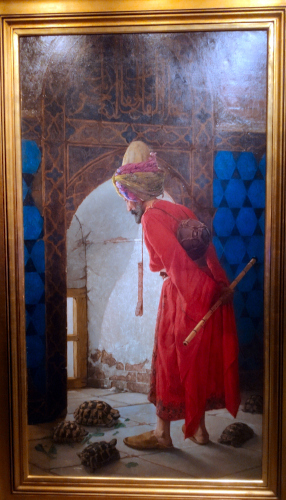
\includegraphics[height=0.95\textheight]{assets/kaplumbaga_terbiyecisi.jpg}
    \caption{Osman Hamdi Bey'in Kaplumbağa Terbiyecisi Tablosu}
\end{figure}